\begin{pastexam}[label={px:ncku-114-isec-ds-18}]{成大智慧資安學程 114 學年度 簡答題第 2 題}
（追蹤）

(10 PTs) Given a graph shown in Fig 2, please answer the following questions:

a) which are the articulation points, and

b) the biconnected components of the graph.

\begin{center}
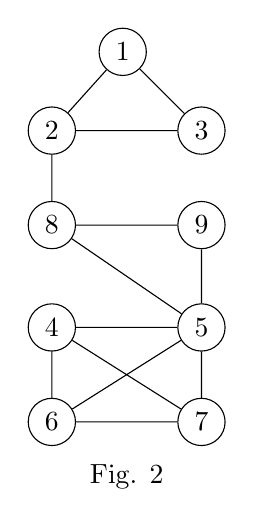
\begin{tikzpicture}[v/.style={draw,circle,minimum size=6mm,inner sep=0pt}]
  \node[v] (1) at (0.9,0) {1};
  \node[v] (2) at (0,-1) {2};
  \node[v] (3) at (1.9,-1) {3};
  \node[v] (8) at (0,-2.2) {8};
  \node[v] (9) at (1.9,-2.2) {9};
  \node[v] (4) at (0,-3.5) {4};
  \node[v] (5) at (1.9,-3.5) {5};
  \node[v] (6) at (0,-4.7) {6};
  \node[v] (7) at (1.9,-4.7) {7};
  \draw (1) -- (2) (1) -- (3) (2) -- (3) (2) -- (8) (8) -- (9) (8) -- (5) (9) -- (5)
        (4) -- (5) (4) -- (6) (4) -- (7) (5) -- (6) (5) -- (7) (6) -- (7);
  \node at (0.95,-5.4) {Fig. 2};
\end{tikzpicture}
\end{center}
\end{pastexam}

\begin{pastsoln}
答案：a) 割點是 $2, 5, 8$。 b) 雙連通元件有四個：$\{1, 2, 3\}$、$\{2, 8\}$、$\{5, 8, 9\}$、$\{4, 5, 6, 7\}$。

圖的邊：$1$--$2$、$1$--$3$、$2$--$3$、$2$--$8$、$8$--$9$、$8$--$5$、$9$--$5$、$4$--$5$、$4$--$6$、$4$--$7$、
$5$--$6$、$5$--$7$、$6$--$7$。

\textbf{用 DFS 的 low 值求}（資結書第~23.5、23.6~節）。 從 $1$ 開始，鄰居照編號由小到大，$\mathit{dfn}$ 是
發現順序，$\mathit{low}(u)$ 是 $u$ 的子樹經過最多一條後向邊能到的最小 $\mathit{dfn}$。
\begin{center}
\small
\begin{tabular}{lccccccccc}
\toprule
頂點 & 1 & 2 & 3 & 8 & 5 & 4 & 6 & 7 & 9 \\
\midrule
$\mathit{dfn}$ & 1 & 2 & 3 & 4 & 5 & 6 & 7 & 8 & 9 \\
DFS 樹的父節點 & -- & 1 & 2 & 2 & 8 & 5 & 4 & 6 & 5 \\
後向邊 & & & 3--1 & & & & 6--5 & 7--4、7--5 & 9--8 \\
$\mathit{low}$ & 1 & 1 & 1 & 4 & 4 & 5 & 5 & 5 & 4 \\
\bottomrule
\end{tabular}
\end{center}
走法：$1 \to 2 \to 3$（$3$ 有後向邊到 $1$），回到 $2$ 再走 $8 \to 5 \to 4 \to 6 \to 7$（$7$ 有後向邊到 $4$、$5$，
$6$ 有後向邊到 $5$），回到 $5$ 再走 $9$（後向邊到 $8$）。 $\mathit{low}$ 由下往上算，例如
$\mathit{low}(7) = \min(8, \mathit{dfn}(4), \mathit{dfn}(5)) = 5$，$\mathit{low}(5) = \min(5, \mathit{low}(4), \mathit{low}(9)) = \min(5, 5, 4) = 4$。

\textbf{a) 割點。} 根 $1$ 在 DFS 樹裡只有一個子節點 $2$，不是割點。 非根的 $u$ 是割點，若且唯若它有子節點
$w$ 滿足 $\mathit{low}(w) \ge \mathit{dfn}(u)$（資結書定理~23.9）：
\begin{itemize}
\item $2$：子節點 $8$ 的 $\mathit{low} = 4 \ge 2$，是割點。 （子節點 $3$ 的 $\mathit{low} = 1 < 2$。）
\item $8$：子節點 $5$ 的 $\mathit{low} = 4 \ge 4$，是割點。
\item $5$：子節點 $4$ 的 $\mathit{low} = 5 \ge 5$，是割點。 （子節點 $9$ 的 $\mathit{low} = 4 < 5$。）
\item $3, 4, 6, 7, 9$：$3, 7, 9$ 是葉子；$4$ 的子節點 $6$ 的 $\mathit{low} = 5 < 6$；$6$ 的子節點 $7$ 的
$\mathit{low} = 5 < 7$。 都不是。
\end{itemize}
直接檢查也一樣：拿掉 $2$，$\{1, 3\}$ 和其他點斷開；拿掉 $8$，$\{1, 2, 3\}$ 斷開；拿掉 $5$，$\{4, 6, 7\}$ 斷開
（它們只經過 $5$ 連到 $8$、$9$）。 拿掉其他任何一點，圖仍連通。

\textbf{b) 雙連通元件。} 每個滿足 $\mathit{low}(w) \ge \mathit{dfn}(u)$ 的樹邊 $(u, w)$，連同 $w$ 的子樹裡還沒
分出去的邊，構成一個元件（資結書虛擬碼~23.4 用邊的堆疊做這件事）：
\begin{itemize}
\item $(5, 4)$：$\{4, 5, 6, 7\}$，邊 $4$--$5$、$4$--$6$、$4$--$7$、$5$--$6$、$5$--$7$、$6$--$7$。
\item $(8, 5)$：$\{5, 8, 9\}$，邊 $8$--$5$、$5$--$9$、$9$--$8$。
\item $(2, 8)$：$\{2, 8\}$，只有一條邊 $2$--$8$（它是橋）。
\item $(1, 2)$：$\{1, 2, 3\}$，邊 $1$--$2$、$2$--$3$、$3$--$1$。
\end{itemize}
十三條邊各屬於恰好一個元件（$6 + 3 + 1 + 3 = 13$）。 割點 $2, 5, 8$ 都同時屬於兩個元件，其他頂點只屬於
一個。
\end{pastsoln}
